\documentclass[12pt]{article}
\usepackage{bookmark}
\usepackage{graphicx} 
\usepackage[german]{babel}
\usepackage{geometry}                % See geometry.pdf to learn the layout options. There are lots.
\geometry{letterpaper}                   % ... or a4paper or a5paper or ... 
\usepackage{graphicx}
\usepackage{amssymb}
\usepackage{amsthm}
\usepackage{epstopdf}
\usepackage[utf8]{inputenc}
\usepackage[usenames,dvipsnames]{color}
\usepackage[table]{xcolor}
\usepackage{hyperref}
\DeclareGraphicsRule{.tif}{png}{.png}{`convert #1 `dirname #1`/`basename #1 .tif`.png}

\theoremstyle{definition}
\newtheorem{example}{Example}

\newenvironment{explanation}{%
   \setlength{\parindent}{0pt}
   \itshape
   \color{blue}
}{}

\newcommand{\projectname}{Ship4You}
\newcommand{\productname}{Ship4You}
\newcommand{\projectleader}{Alexander Hrazdera/Paul Schöffl}
\newcommand{\documentstatus}{In Arbeit}
%\newcommand{\documentstatus}{Submitted}
%\newcommand{\documentstatus}{Released}
\newcommand{\version}{V. 1.0}

\begin{document}
\begin{titlepage}

\vspace{10em}

\begin{center}
{\Huge Project Proposal} \\[3em]
{\LARGE \productname} \\[3em]
\end{center}

\begin{flushleft} 
\begin{tabular}{|l|l|}
\hline
Projekt Name & \projectname \\ \hline
Projekt Leiter & \projectleader \\ \hline
Dokumenten Status & \documentstatus \\ \hline
Version & \version \\ \hline
\end{tabular}
\end{flushleft}

\end{titlepage}
\section*{Revisions}
\begin{tabular}{|l|l|l|}
\hline
\cellcolor[gray]{0.5}\textcolor{white}{Date} & \cellcolor[gray]{0.5}\textcolor{white}{Author} & \cellcolor[gray]{0.5}\textcolor{white}{Change} \\ \hline
September 19, 2019&A. Hrazdera/P. Schöffl&First version \\ \hline
\end{tabular}

\pagebreak

\tableofcontents

\pagebreak

\section{Einführung}
Das Ziel dieses Projektes ist es, eine Website für Segel oder Motoryachten (Boote) zu erstellen. Der Sinn dieser Website ist es, die Boote zur Bewertung freizugeben. Somit kann jeder User der sich ein Boot mieten möchte (egal wo) ein gutes Bild über den Vermieter und den Zustand des Bootes machen. Es kann nicht mehr passieren, dass man von einem Vermieter (Charterer) über den Tisch betrogen wird. Auch kann man sich so leichter mit den Vermietern zusammenschreiben. Weil es so ein Produkt noch nicht auf dem Markt gibt kann man die Idee auch leicht erweitern und vermarkten. 

\pagebreak

\section{Ausgangssituation}
Aktuell kann beim Anmieten einer Yacht oder eines Segelbootes auf das Angebot verschiedener Vermieter (Charterer) nur so zugegriffen werden, dass der Mieter die einzelnen Websiten der Charterer besucht und sich das Angebot ansieht. Eine globale Suche von Booten in einer bestimmten Region ist derzeit nicht möglich.

Weiters ist es noch nicht möglich, eine unabhängige Bewertung der Geschäfts\-trans\-aktion einer Vermietung (Zustand des Boots, Qualität der Betreuung, etc.) einzusehen. So ist man derzeit als Mieter noch von den Angaben des Vermieters abhängig und es ist schwierig bis unmöglich, sich ein eigenes und unabhängiges Bild zu machen. Dies gilt sowohl für die textuelle Beschreibung des Bootes als auch für die zur Verfügung gestellten Bilder.

Auf der anderen Seite ist es für Charterer auch sehr schwierig ihr Angebot an Booten zu kommunizieren. Jeder einzelne Vermieter muss sein Angebot auf seiner eigenen Website bewerben. Dies impliziert einen signifikanten Aufwand, der vor allem von Kleinvermietern nicht geleistet werden kann.

Im Bereich der Ferienzimmervermietung oder auch Ferienwohnungsvermietung gibt es bereits ein Angebot an zentralen Plattformen (Airbnb, HomeAway, etc), welche einen niederschwellig zugänglichen Marktplatz für die Vermietung von Wohnungen und Zimmer ermöglicht.

\pagebreak

\section{Allgemeine Bedingungen und Einschränkungen}
Solange kein Bezahlservice angeboten wird, genügt die Angabe einer e-mail und eines Benutzernamens. Validierung einer Anmeldung kann über einen Bestätigungslink per e-mail erreicht werden. Weitere persönliche Daten und daraus resultierende Datenoffenlegung sind dann zu untersuchen, wenn ein Bezahlsystem integriert wird.

Das User Interface muss sowohl für angemeldete als auch für anonyme Benutzer zur Verfügung stehen. Vor allem sollten anonyme Benutzer ein ungestörtes Sucherlebnis geboten bekommen, solange sie nicht Boote bewerten wollen. Das GUI hat vor allem in der Gestaltung der Suche eine hohe Komplexität zu bewältigen, da die Suchkriterien sehr vielfältig sind. Beispielsweise sind folgende Suchkategorien relevant:

\begin{itemize}
   \item Auswahl einer oder mehrerer geografischer Regionen
   \item Suche nach dem Typ und dem Namen des Boots
   \item Name des Vermieters
   \item Alter des Bootes
   \item Anzahl der Schlafplätze und/oder Kabinen
   \item Preis
   \item Anzahl der Masten und/oder Segel
   \item Rumpftyp (Einzelrumpf, Katamaran)
   \item Baujahr
   \item Sonderausstattung (Spinnaker, Dingi, Radar, Kartenplotter, Autopilot, Heizung)
\end{itemize}

Bei den anonymen und angemeldeten Benutzer:
\begin{itemize}
   \item Eine weitere Komplexität sind die angebotene Sortierungen, welche nach Preis, nach Beliebtheit, nach geografischer Nähe, nach Namen und Typ des Bootes sein können. Die Sortierung soll einfach und schnell gewechselt werden können.
\end{itemize}

Bei angemeldeten Benutzer:

\begin{itemize}
   \item Im Vordergrund steht auch die einfache Kontaktaufnahme über die E-mail, der Telefonnummer oder einem intigrierten Chat, mit dem Beitrag Ersteller.

   \item Das Hinzufügen von Bewertungen bzw. neuen Booten sollte ziemlich einfach gestaltet sein. Ein Bilder-upload über den Dateiexplorer sollte auch zur Verfügung stehen.
\end{itemize}


Die Anwendung muss mehrsprachig gestaltet werden, weil viele Häfen nicht in Österreich oder Deutschland liegen. Am Anfang wird die Website zweisprachig ausgelegt sein (Deutsch und Englisch).

\pagebreak

\section{Projektziele und Systemkonzepte}
Die Projektziele lassen sich wie folgt zusammenfassen:

Für das Ansehen und Suchen der Boote bzw. der Bewertungen ist keine Anmeldung von nöten. Diese wird nur beim Hinzufügen der Boote bzw. der Bewertungen benötigt.
Zum Anmelden werden ein Benutzername, eine e-mail und ein Passwort benötigt. Dem User wird eine Bestätigungs-email gesendet über diese er sich Verifizieren muss. 
Dem User ist es möglich eine Schnell-Fragestelle aufzurufen, sprich eine Chatseite wo alle, auch die nicht angemeldet sind, fragen zu Booten stellen können und dort Inforamtionen austauschen sollen. Die Fragen können von den jeweiligen Useren mit einem Like oder Dislike bewertet werden. Wenn eine Frage gestellt wurde, kann diese auch wieder bearbeitet oder gelöscht werden.
Durch einen freundlichen und hilfreichen Support kann der Kunde sich auch bei Fragen an das Team wenden.
Das kommunizieren zwischen den Usern erfolgt über einen anonymen Chat (zusehen auf Willhaben.at). Zu den schriftlichen Bewertungen wird auch noch eine Sterne Bewertung zur verfügung gestellt.  

Weiters liegt der Unterschied zwischen der von uns geplantet Website und den schon bestehenden Websiten darin, dass jeder der sich angemeldet hat ein Boot hinzufügen kann. Somit kann ein Mieter das von ihm gemietete Boot hinzufügen und dieses Bewerten (Wie in einem Forum). Dadurch werden schneller Boote online gestellt. Des weiteren sind die Bewertungen dann ehrlicher.\\\\
Vorteile für den Besitzer:
\begin{itemize}
\item Der Besitzer, der das Boot als Wirtschaftsfaktor verwendet, erhält direkt vom Mieter entsprechende Informationen über Schäden oder sonstige Rückmeldungen (guter Anker, Komfort, gewählte Ausstattung, Plotter,..)
\end{itemize}
Vorteile für den Vermieter:
\begin{itemize}
\item Der Vermieter bekommt eine bessere Werbung und wird durch bessere Bewertungen wahrscheinlich öfter gebucht.
\item Auch kann sich dieser, über einen bei unserer Website integrierten Chat, mit den Mietern austauschen.
\end{itemize}
Vorteile Für die Mieter:
\begin{itemize}
\item Das Risiko betrogen zu werden sinkt.
\item Man kann sich einen guten Überblick über den Jetzt-Zustand des Bootes machen und kann auch die bisherigen Schäden einsehen.
\item Netter und Hilfreicher Support auf unserer Website
\item Keine Anmeldung um Boote zu suchen.
\end{itemize}


\pagebreak

\section{Chancen und Risiken}
Es bestehen Kontakte des Projektteams zu diversen Segelclubs und Häfen. In einer Umfrage von Verantwortlichen für Segelclubs und Bootsmietern 5 Personen befragt. Davon würden 5 eine derartige Website sofort unterstützen. 

Die Vermarktung wird  darum auch über die verschiedenen Häfen bzw. Segelclubs bereitgestellt.

Das Projekt hat folgende Möglichkeiten:
\begin{itemize}
\item Mieter bekommt für sein Geld das bestmögliche Boot, weil er von anderen Usern die Bewertungen der Boote einsehen kann.
\item Aufgrund der abgegebenen Bewertungen der User zu den Booten und dem Charterer, sinkt das Betrugsrisiko beträchtlich. Des weiteren helfen einem die hochgeladenen Bilder und Kommentare sich ein gutes Bild über das Boot zu machen.
\item In weiterer Folge ist es sicherlich auch eine Erleichterung für den Vermieter. Dieser bekommt einen weiteren Platz sein Boot zu bewerben und erhält gleichzeitig ein konstruktives, hoffenlich gutes Feedback.
\item Aufgund reger Nachfrage ist auch der Vertreib der Website gesichert.
\end{itemize}

Das folgende Risiko ist zu berücksichtigen:
\begin{itemize}
\item Bewertungen können durch Fehlerhafte Bilder bzw. Kommentare verfälscht werden. Aufgrund der Anmeldung versuchen wir den durch Bots verursachbaren Schaden möglichst klein zu halten.
\end{itemize}

\pagebreak

\section{Planung}
Der erste Meilenstein wird die Erstellung der Haupseite und der UI sein diese wird bis zum 1 Dezember 2019 abgeschlossen sein.
Die UI sollte modern und einfach gestaltet sein. Auf der Startseite wird sich die Suche nach dem Standort und dem Namen eines Bootes befinden. Dem User werden das gesuchte Boot, die Bewertungen bzw. Kommentare dazu auf dem ersten Blick angezeigt. Nun kann er sich mit anderen Leuten darüber austauschen. Auch kann er sich bei Fragen an die Community oder direkt an den Charterer wenden. 
Der zweite Meilenstein wird das Anmelden der Benutzer sein dieser wird bis zum 2 Februar beendet sein. Dieser Punkt ist für die Vermieter wichtig. Er kann somit sein Boot auf diese Website stellen. Auch ist diese Funktion wichtig für Benutzer die das Boot schon gemietet haben und eine Bewertung für dieses Boot abgeben möchten.
Als drittes folgt eine Datenbank mit den ganzen Häfen bzw. Booten, hierbei ist es wichtig, das die Daten schnell und ohne Probleme zur Verfügung stehen. Beendet wird dieser am 1 April 2020 sein. 
Der vierte Meilenstein ist für die Suche dieser Häfen bzw. Boote zuständig dieser wird bis zu 1 Mai 2020 fertig sein. Auch hier darf die Suche nicht zu lange dauern. Um diese Daten zu finden wird die Datenbank durchsucht.
\\ Alexander Hrazdera und Paul Schöffl sind für die Dokumentation und der Erstellung der Website zuständig.\\ Wir benötigen 2 Programmierer mit jeweils einem eigenen Notebook. Einen Server mit einer Datenbank und eine Websitedomain wird auch benötigt.
\\
\\
\begin{center}
\section*{Registrieren und Login}
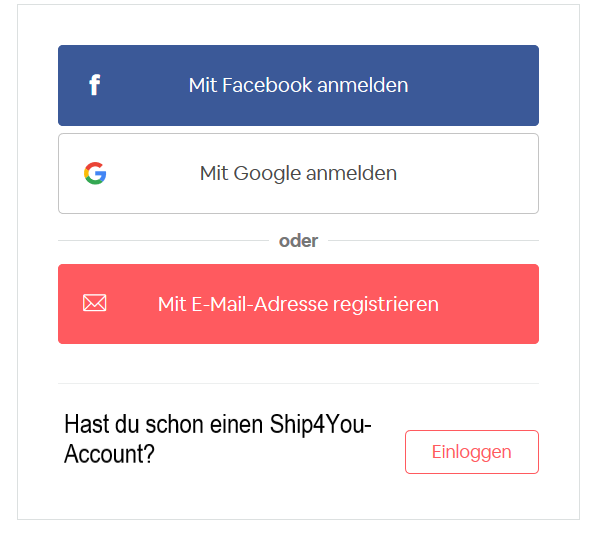
\includegraphics[height=0.50\textwidth]{Login.png}
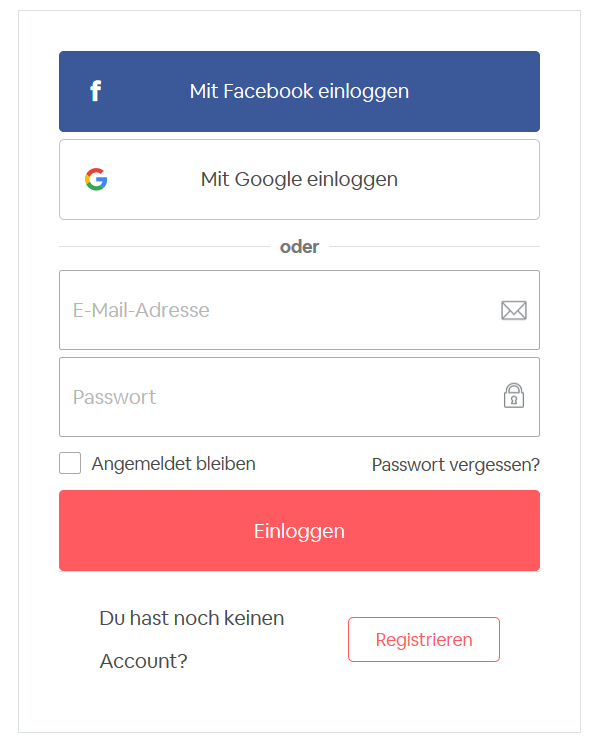
\includegraphics[height=0.50\textwidth]{Login2.PNG}
\section*{Startseite- Suchfunktion}
\end{center}
\begin{center}
\includegraphics[width=15cm,height=20cm,keepaspectratio]{Startseite2.png}\end{center}
\begin{center}
   \section*{Filtern nach Booten}
   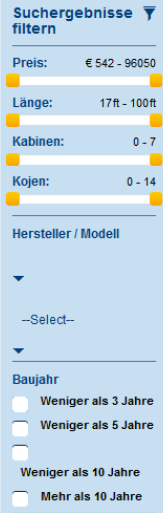
\includegraphics[height=0.80\textwidth]{Filter1.PNG}
   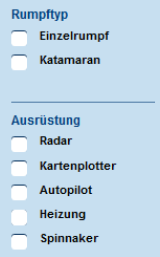
\includegraphics[height=0.80\textwidth]{Filter2.PNG}
\end{center}
\pagebreak
\newcommand{\projektend}{30 Juni 2020}
\newcommand{\projectstart}{23 September 2019}
\newcommand{\firstresult}{Ende Jänner}
\newcommand{\beginofprog}{7 Oktober}
\newcommand{\bigBlocks}{Design der Website/der Login/Datenbankerstellung}
\newcommand{\whatisneeded}{Datenbank/Websitedomain}

\begin{flushleft} 
\begin{tabular}{|l|l|}
\hline
Projekt Ende: & \projektend \\ \hline
Projekt Start: & \projectstart \\ \hline
Erster fertiger Prototyp: & \firstresult \\ \hline
Beginn der Umsetzung: & \beginofprog \\ \hline
Größten Blöcke: & \bigBlocks \\ \hline
Was wird benötigt? & \whatisneeded \\ \hline
\end{tabular}
\end{flushleft}
\cite{endLine}
\bibliography{my_bib}{}
\bibliographystyle{plain}
\end{document}  